\subsection{Andrew DeGarmo}
\underline{Role:} I chose to attend every meeting we had with questions, concerns, and ideas about the project goal so we could outline the team’s objectives clearly. 
As a group, we ensured each member was on the same page. 
I kept track of our budget and the amount we had spent. 
Although the roles in the team weren’t clearly defined, we equally shared responsibilities such as ordering materials, tracking the budget, setting our achievable goals before the next meeting, and brainstorming ideas during meetings.

\underline{Tasks Completed:} The tasks I completed during this semester were sharing thoughts and ideas contributing to the goals of our project. 
I attended all meetings and ensured we were all on the same page before dismissing–having a clear understanding of our roles and responsibilities before meeting again was important to clear up confusion among the members. 
I ordered the parts for the current clamp and designed the hardware architecture, software architecture, and system functionality diagram. 
I contributed to the overall architecture design at the beginning of the semester. 
I contributed to the design choices throughout the semester and wrote the design choices section in the Final Report. 
I also completed the Overall architecture, Hardware architecture, Software architecture, and Timeline sections. 
The last design I completed was to create the wire for the current clamp. 
I created a pinout architecture from the GPS and the Raspberry Pi.

\underline{Results:} The architectures from Figure 4 shown above were modeled to create the Raspberry Pi and its hardware connections necessary to finish the hardware portion of our project. 
Interfacing the current clamp onto the Raspberry Pi and GPS module correctly required knowledge of the Pi and GPS pinout. 
Figure 7 represents this pinout configuration and was used to connect the current clamp Pi hat to the Raspberry Pi.

\begin{center}
    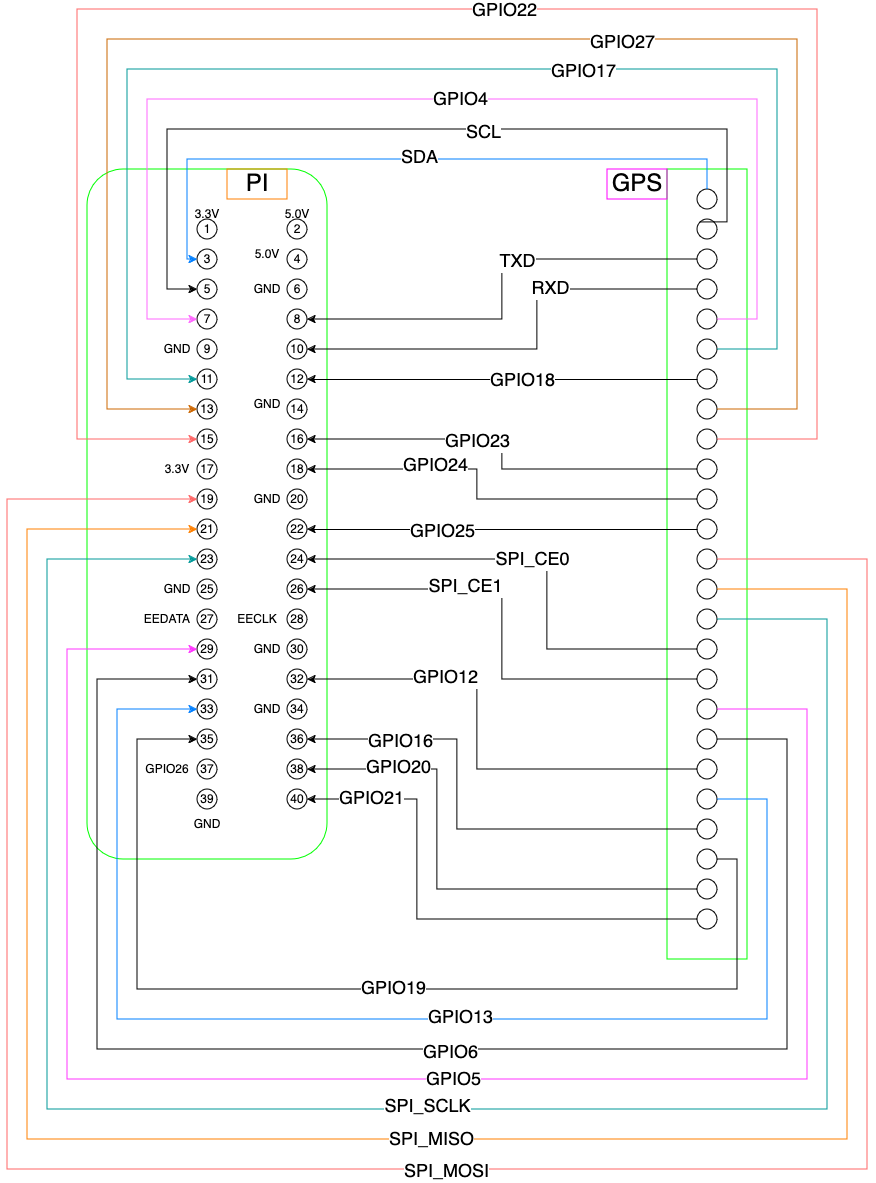
\includegraphics[width=0.5\textwidth]{Pin_Diagram.png}\\
    Fig 7. Raspberry Pi to GPS pinout
\end{center}

\subsection{Samesh Desai}

\subsection{Emma Kupec}
\underline{Role:} My role within the team was not consistent. 
I would consider myself to be one of the organizers, however most often we shared responsibilities. 
Within the team, I often found myself taking charge of being aware of the goals we needed to achieve and helping to facilitate the completion of such goals. 
My role as a designer was shared this semester with nearly all of my team members, as we mostly contributed equally to brainstorm sessions and communicated as a group about decisions regarding our proposed design.

\underline{Tasks Completed:} The following tasks completed this semester were a collaborative effort. 
At the beginning of the semester I helped facilitate initial contact with our mentor and proposed many ideas for how to get started with the project. 
Throughout the designing process, I contributed equally to group brainstorming sessions, discussions, build days, and test days. 
I was available to work on class assignments and made sure I was reviewing group work to ensure an optimal product.

\subsection{Kevin Meyers}

\subsection{Omar Ndiaye}
\underline{Role:} As a team member, my role was versatile, adapting to the needs of the project as they arose. 
Primarily, I focused on ensuring my tasks were completed efficiently and effectively. 
This involved actively listening to project requirements and trying to get it done before the due date. 
Additionally, I contributed to group brainstorming sessions by listening to different ideas and trying to implement them, and I also tried to be very collaborative and have an understanding approach to all project activities.

\underline{Tasks Completed:} For this assignment I contributed to the tasks in a collaborative effort with the team. 
As the project progressed, I participated in some group brainstorming sessions, discussions. 
I ensured to get some of my team members to review my group work to maintain the quality and get fresh ideas on what more to include. 
For this assignment I completed the risk, and test plans section with the GPS Data Visualization Proof of Concept and Current Clamp Testing with Space Heater.

\subsection{Greyson Weimer}
\underline{Role:} My role within the team was primarily technical, leveraging my breadth of knowledge across Electrical Engineering, Computer Engineering, Computer Science, and Cybersecurity.
I helped with planning and designing the current clamp measurement system.
I have extensive knowledge of Linux, and this came in handy when designing our remote access and remote management system.
I have a love for LaTeX and thus converted all of our deliverables into LaTeX formatted PDFs.

\underline{Tasks Completed:} For this assignment I was not able to contribute as much as I would have liked due to personal issues.
I was primarily focused on doing the conversion to LaTeX, as well as helping out with general grammar and technical editing.
For the other assignments, I made sure to share equal responsibility.
Throughout the project I helped a lot with research for the Pi HATs, determining which ones to get, what libraries and code we could use to use them, as well as soldering the current clamp circuit together.
